\documentclass[letterpaper,10 pt,conference]{ieeeconf}

\IEEEoverridecommandlockouts
\overrideIEEEmargins

\usepackage[utf8]{inputenc}
\usepackage[T1]{fontenc}

\usepackage{graphics} % for pdf, bitmapped graphics files
%\usepackage{mathptmx} % assumes new font selection scheme installed
\usepackage{times} % assumes new font selection scheme installed
\usepackage{amsmath} % assumes amsmath package installed
\usepackage{amssymb}  % assumes amsmath package installed
\usepackage[backend=bibtex8,style=ieee,sorting=none]{biblatex}

\usepackage{graphics} % for pdf, bitmapped graphics files
\usepackage{caption}
\usepackage{subcaption}
\usepackage{standalone}
\usepackage{tikz}
\usepackage{tikzscale}
\usetikzlibrary{calc}

\graphicspath{{img/}}
\addbibresource{references.bib}

\title{\LARGE \bf
  Optimizing Topometric Maps for Teach and Repeat
}


\author{David Landry and Alexandre Gari\'epy}


\begin{document}

\maketitle
\thispagestyle{empty}
\pagestyle{empty}


\begin{abstract}

  abstract

\end{abstract}

\section{INTRODUCTION}

Teach and Repeat is a popular and efficient paradigm to execute tasks where it is possible to have
an operator show the robot how to execute the task beforehand. It has been implemented using stereo cameras
\cite{Furgale10} or lidar sensors \cite{Sprunk13}.

\begin{itemize}
    \item Talk about teach and repeat
    \item How teach maps are aquired (point clouds are taken at regular steps)
    \item Why we want to optimize this (loop closure spped, memory for large maps)
\end{itemize}


\section{RELATED WORK}


\section{PROBLEM DEFINITION}

In our current implementation of the Teach and Repeat paradigm, the maps we use to repeat a
trajectory contains anchor points, transformations to go from one anchor to another, as well as
recorded commands for the whole trajectory. This paper, however, is focused on how to improve the
size of the underlying topometric map, without consideration for the list of commands.

We begin with an unoptimized topometric map, containing $N$ a set of interconnected nodes and $T$
the geometric transformations to go from one node to it's neighbor. The nodes in $N$ are in fact
anchor points to our teach an repeat implementation. They are point clouds in this case, but could
be any mean of localization, like features in an image. Every node $n_i$ has an associated point
cloud $p_i$. The nodes are linked as a chain, from the first node recorded to the last.

Our objective is to find the smallest subset of $N$ such that the robot can reliably localize itself
against a node at any time while it follows the taught trajectory. To decide wether the robot can
localize itself at a given position on the taught trajectory, we will induce an error in the
transformation estimate between both nodes. The intuition behind it is that by inducing increasingly
large errors, and having the ICP succeed nontheless, we can guarantee an increasingly large
robustness by going in the field. When the induced error becomes large enough, the localisation will
fail: the ICP algorithm will enter a local minimum, and the result of the ICP will be largely
different that the induced error.

\section{OUR APPROACH}
\label{approach}

\subsection{Deciding if a reading and anchor point pair can be used for localization}
\label{approach-deciding-converge}

First, lets define the terms reading and anchor point:

\begin{itemize}
  \item \textbf{Anchor point:} an anchor point is a node $n_i$ the nodes of the unoptimized topometric map. Each
    anchor point has an associated point cloud $p_i$. This point cloud is used as the reference point cloud when performing the
    ICP algorithm.
  \item \textbf{Reading:} a reading is the point cloud produced by the robot sensor during the repeat phase. However,
    we do the optimization of the topometric map in an offline process using only the teach data. Therefore,
    we use simulated reading. To simulate a reading, we take the point cloud $p_j$ of an anchor point and induce an
    error. This error is a 2D translation vector $[x, y]^T$, where $x$ is the forward-backword error and $y$ is the left-right error,
    following ROS frame convensions.
\end{itemize}

Lets consider a reading $r$ and an anchor point $a$. We know that $r$ is derived from inducing an error $[x, y]^T$ to $p_r$, which is associated to a node $n_r$.
We also know that the anchor point $a$ is associated to a node $n_a$ and a point cloud $p_a$. We can easily get the transform $t$ between $n_r$ and $n_a$ from $T$.


We want to know if the $a$ can be used to localize $r$. To do so, we run the ICP algorithm using $r$ as the input and $p_a$ as the reference, using $t$
as the initialization of the ICP. ICP returns a transform $[x_{icp}, y_{icp}]^T$. We would except that ICP corrects the induced error by returning
a transformation $[-x, -y]^T$. This is verified by checking if the norm of the vector $[x_{icp}, y_{icp}]^T - [-x, -y]^T$ is under a certain $\epsilon$.


\subsection{Convergence ellipse}
Given two nodes $n_i$ and $n_j$ in $N$, we can use $n_i$ to generate readings and $n_j$ as an anchor point.
We define the concept of a convergence ellipse as the ellipse around $n_i$ where we generate readings by inducing
error corresponding to the position in the ellipse, the center of the ellipse being no induced error. We call the ellipse
a convergence ellipse because each generated reading can be used for localization using the $n_j$ anchor point, as described in the
section \ref{approach-deciding-converge}


The ellipse has been choosen because it is a geometric shape that fits well the convergence bassin, or zone where we can induce error and the ICP still
converges (see figure \ref{convergence_bassin}). We also observed that this zone is continuous; there is no ``hole'' where the ICP doesn't converge inside the bassin.
Therefore, we only need to test readings on the circonference to verify if an ellipse is a convergence ellipse.

\subsection{Mapping matching readings}

\subsection{Topometric map as a graph}

\subsection{Smallest topometric map}

\begin{itemize}
  \item Choose elipse of a given shape. We assume that if ICP converges on the
    ellipse, it would converge at any given point inside the ellipse (we need the explain why we made this assumption)

  \item For each point, find the nearest point that doesn't converge with ICP

  \item Create an oriented graph where arcs represents a successful ICP convergence

  \item Find the shortest path in the graph from that converge

\end{itemize}

\begin{figure}
  \centering
  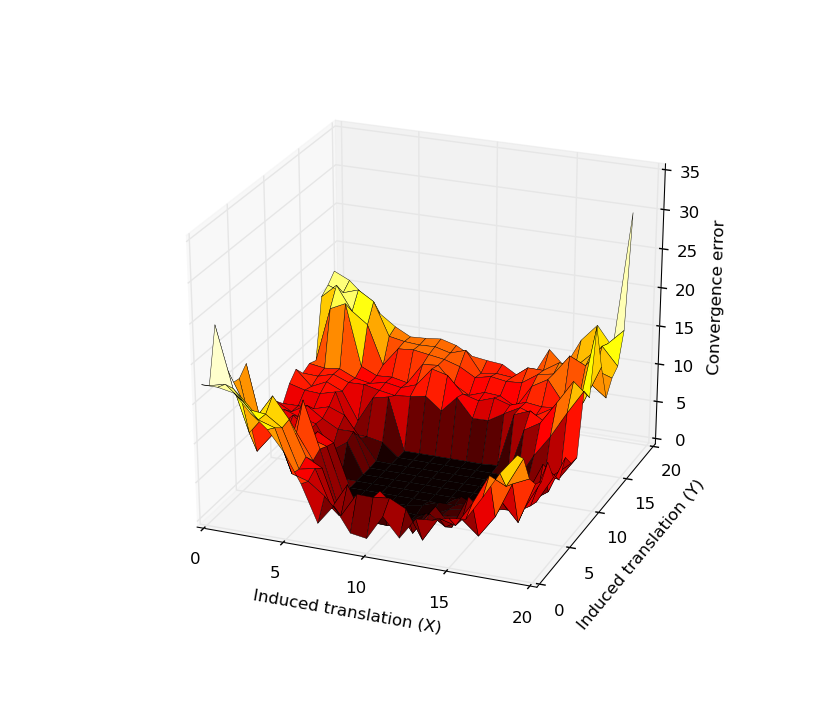
\includegraphics[scale=0.4]{convergence_bassin}
  \caption{The covergence bassin of a pair of readings}
  \label{convergence_bassin}
\end{figure}


\begin{figure}[thpb]
  \centering
  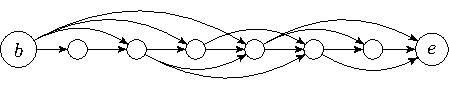
\includegraphics[scale=1.0]{unoptimized-graph}
  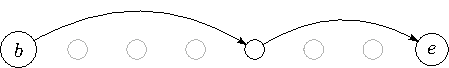
\includegraphics[scale=1.0]{optimized-graph}
  \caption{Optimal node subset using the graph approach}
\end{figure}


\section{EXPERIMENTS}
We can talk about the offline optimisation we did on some dataset.

\begin{figure}
  \centering
  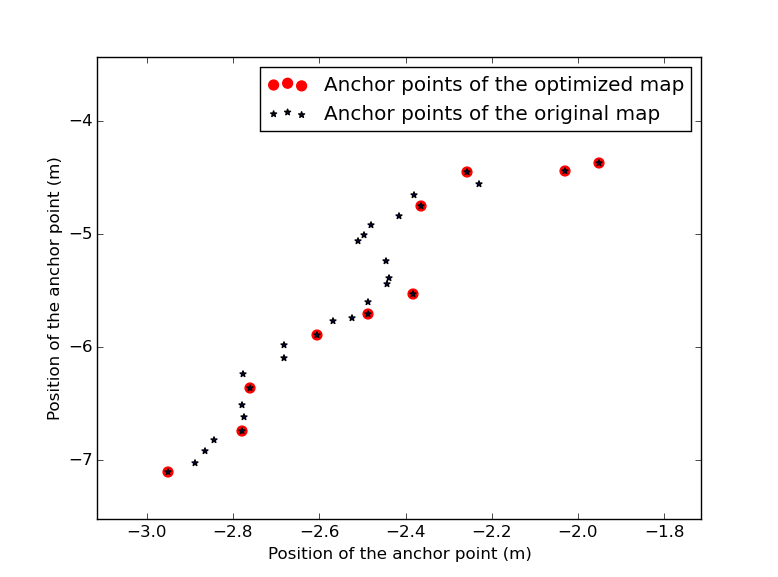
\includegraphics[scale=0.4]{map_optimization}
  \caption{Comparison of un-optimized and optimized maps}
\end{figure}

First we ran our approach on three dataset from previous \textit{teach} sessions. The
\textit{terasse} dataset is a short run paving stones on Université Laval's campus. It was a busy
summer day, and passer-by that were curious about the robot introduced noise in the point
clouds. The \textit{forest} dataset is a short run in some woodland on campus, making the environment
highly unstructured. Finally, we used \textit{hallway}, mapping an indoor hallway, as a
benchmark through the development of the algorithm. It records the robot going in a straight line.
During this \textit{teach} session the robot was tuned to record a very high number of point clouds,
so we expect the optimization algorithm to filter a lot of nodes in this case.

We used parameters $a=0.4 m$, $b=0.4 m$ and $\epsilon=0.05 m$ for those optimization runs. The
optimization is indeed able to reduce the number of point clouds necessary to execute a
\textit{repeat} session. As exepected, depending on the robot trajectory some zones contain more
superfluous nodes than others. Straight lines in very static environments tend to require less
anchor points, where trajectories containing heavy rotations are less filtered out. The algorithm
tends not only to eliminate superfluous point clouds, but it also gets rid of the nodes that are
hard to localize against, for instance a point cloud containing a passer-by that is not there on the
other neighboring point clouds. For instance in the \textit{hallway} dataset, even though the
overall localization using ICP is easy, some clouds could not be used for localization at all.
Finally, the number of remaining nodes could be tuned down even more, at the cost of a lower
tolerance to error. Our algorithm thus gives the user a very direct way to control the
memory-size/ability-to-localize tradeoff. The numbers given in table
\ref{tabopti} are meant to give a general idea, but they could be very different depending on the
geometry of the environment, the parameters given by the user, and the quality of the odometry
estimates.

We noticed that in some datasets, the \textit{ICP chain} used to reconstruct the relative positions
between the nodes may be noisier than we thought, yielding unrealistic positions for sucessive
anchor points. It leaves us wondering wether we should rather rely on the odometry from the weels as
a reference transformation. A Kalmann Filter using both odometry and the results from ICP would be
optimal.

\begin{table}[h]
\centering
\begin{tabular}{|l|r|r|r|}
  \hline
Dataset & N. of points & N. of points after optimization & \% \\
\hline
terasse & 304 & 186 & 61.2 \\
  \hline
forest & 62 & 41 & 66,1 \\
  \hline
\end{tabular}
\caption{The result of the optimization on different datasets}
\label{tabopti}
\end{table}

\section{FUTURE WORK}

\subsection{Experiment with Husky}

\subsection{Multi-objective optimization for automatic parameter selection}

To focus our efforts on fiding the minimal node subset, we made the simplication the convergence ellipse has a fixed sized.
has a fixed sized.  In other words, we manually specify the distance in $x$ and $y$ for which we
want the ICP to converge. With those parameters given, we can reduce the problem to a finding the
shortest path in a graph, as shown in section \ref{approach}.


A limitation of this approach is that, if for a given node, decreasing the size of the ellipse would
make the ICP converge on further nodes of the graph. We can see that as a tradeoff between the
precision and the number of nodes of the final map.


An improvement on the current method would be model the problem as a multi-objective optimization
problem. Given an initial ellipse size for each node of the graph, changing reducing the size of the
ellipse has a cost. The goal is to find the best tradeoff between the length of the shortest path in
the graph and the the costs of the nodes that are used by that shortest path.

\subsection{Handling rotations}

For the sake of simplicity we did not use rotations when inducing errors to the reading's
position estimate, before testing the reliability of the localization. To make the optimization
problem more difficult, while giving the user more ways garantee the reliability of the optimized
maps, we could replace $T$ the space of translations with $R \times T$ the space of rotations and
translations in function $f$. That way, the user could demand that the generated maps be tolerant to
a certain error in the orientation of the robot.

Using the whole space of rotations $R$ might be too general, as it is often useful to simplify the pose of a
ground robot begin a vector $[x, y, \theta]^t$, $\theta$ being the heading. That case could also be
handled by replacing the tolerance ellipse by an ellipsoid. The supplementary dimension would
represent the error in heading, or $\Delta \theta$.

\subsection{Reoptimization of the localizability graph}

The optimization could be taken a step further if we make one more assumption about the behavior
of the \textit{repeat} phase. So far we assumed that the repeat algorithm would work that way: when
following a trajectory passing by anchor points $a$ then $b$, the robot would use point $a$ as a
reference for localization until it is very close to $b$, and then switch reference. It would be
reasonable to have the robot behave differently and make it switch references somewhere in between
$a$ and $b$, which would make the localization easier.

This modification would allow us to make an even better optimization of the topometric maps. When
finding the shortest path in the localizability graph, we ensure that every node in the graph can be
reached by using the preceding node as a reference. This means (assuming that the ICP algorithm is
reflexive) that every second anchor point in our optimized map becomes superfluous and can be removed.

\section*{REFERENCES}
\printbibliography

\end{document}
